% ***************************************** SYMBOLS
\def\abs#1{\lvert#1\rvert}
\def\argdot{{\hspace{0.18em}\cdot\hspace{0.18em}}}
\def\avg#1{\left\{#1\right\}_\omega}
\def\D{{\tn D}}
\def\div{\operatorname{div}}
\def\Eh{\mathcal E_h}       % edges of \Th
\def\Ehcom{\mathcal E_{h,C}}         % edges of \Th on interface with lower dimension
\def\Ehdir{\mathcal E_{h,D}}         % Dirichlet edges of \Th
\def\Ehint{\mathcal E_{h,I}}       % interior edges of \Th
\def\grad{\nabla}
\def\jmp#1{[#1]}
\def\n{\vc n}
\def\vc#1{\mathbf{\boldsymbol{#1}}}     % vector
\def\R{\mathbb R}
\def\sc#1#2{\left(#1,#2\right)}
\def\Th{\mathcal T_h}       % triangulation
\def\th{\vartheta}
\def\tn#1{{\mathbb{#1}}}    % tensor
\def\Tr{\operatorname{Tr}}
\def\where{\,|\,}
%***************************************************************************

\section{Reaction term in transport}
\label{sec:reaction_term}

We have not mentioned yet details about the reaction term $F_R(c^1,\ldots,c^s)$ on the right hand side of the equation (\ref{e:ADE}).
There are several models which can be considered in this reaction term, both of chemical or physical nature. 
The figure \ref{fig:reaction_term} shows all possible reactional models that we support in the trasport process. The Operator Splitting method enables 
us to deal with the convection part and reaction term side by side. The convected quantities do not influence each other in the convectional
process and are balanced over the elements. On the other hand the reaction term relates the convected quantities and can be computed 
separately on each element.

We move now to the description of the reaction term models which can be seen again in the figure \ref{fig:reaction_term}. 
The convected quantity is considered to be the concentration of substances. 
Up to now we can have \emph{dual porosity}, \emph{adsorption} (these two are more of a physical nature) and \emph{reaction} (we mean chemical 
reaction) models in the reaction term. 

\begin{figure}
  \centering
  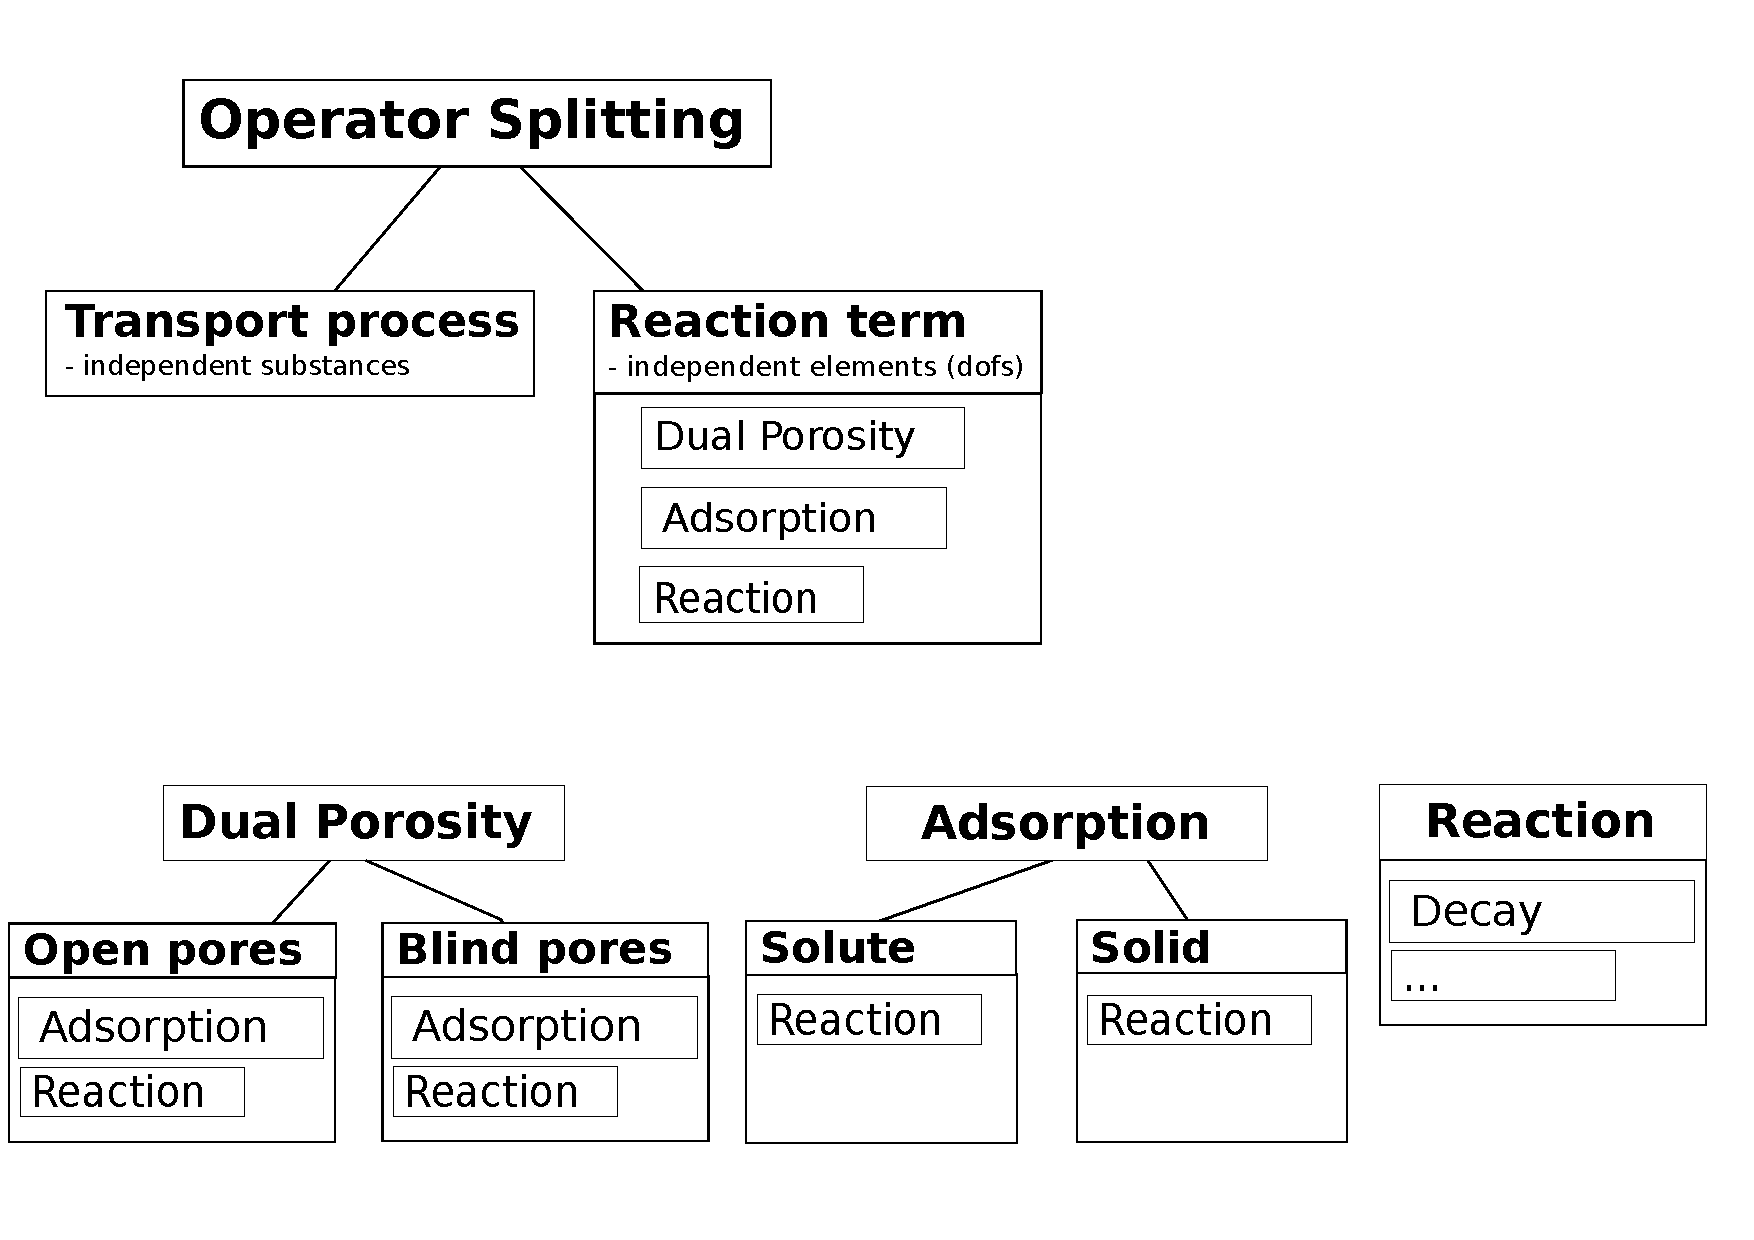
\includegraphics[width=\textwidth]{\fig/reaction_term.pdf}
  \caption{The scheme of the reaction term objects. The lines represents connections between different models. 
  The tables under model name include the possible models which can be connected to the model above.}
  \label{fig:reaction_term}
\end{figure}

The \emph{reaction} model computes chemical reactions on the substances involved. It does not have any additional output.

The \emph{adsorption} model describes the exchange of concentration of the substances between liquid and solid. It can be
followed by a chemical \emph{reaction} that can run in both phases. The concentration in solid is an additional output 
of this model. See the subsection \ref{sec:sorp_math}.


The \emph{dual porosity} model, described in the subsection \ref{sec:dual_porosity}, introduces so called immobile pores in the matrix
which are dead-end pores. The convection process operates only on the concentration of the substances in the mobile zone (open pores) 
and the exchange of concentrations from/to immobile zone is governed by molecular diffusion. This process can be followed by 
\emph{adsorption} model and/or chemical \emph{reaction}, both in mobile and immobile zone. The immobile concentration is saved
in addition.


\subsection{Dual porosity.}
\label{sec:dual_porosity}

Up to now we have described the transport equation for the single porosity model. The dual porosity model splits the mass into 
two zones -- the mobile zone and the immobile zone. Both occupy the same macroscopic volume, however on the microscopic scale, 
the immobile zone is formed by the dead-end pores, where the liquid is trapped and cannot pass through. The rest of the pore volume 
is occupied by the mobile zone. Since the liquid in the immobile pores is immobile, the exchange of the substance is only due 
to molecular diffusion. We consider simple nonequilibrium linear model:
\begin{align}
    \vartheta_m \partial_t c_m &= D_{dp} ( c_i - c_m), \label{eqn:dual_porosity_ode1}\\
    \vartheta_i \partial_t c_i &= D_{dp} ( c_m - c_i), \label{eqn:dual_porosity_ode2}
\end{align}
where $c_m$ is the concentration in the mobile zone, $c_i$ is the concentration in the immobile zone and
$D_{dp}$ is a diffusion rate (\hyperA{DualPorosity-Data::diffusion-rate-immobile}{$diffusion\_rate\_immobile$}) between the zones.
$\vartheta_i$~denotes porosity of the immobile zone (\hyperA{DualPorosity-Data::porosity-immobile}{$porosity-immobile$}) and 
we set the mobile porosity equal $\vartheta_m = \vartheta$ from transport equation (\ref{e:ADE}) which is given by
\hyperA{TransportOperatorSplitting-Data::porosity}{$porosity$}.

The analytical solution of the system of differential equations at time $t$ with initial conditions $c_m(0)$ and $c_i(0)$ is
\begin{align}
     c_m(t) &= (c_m(0) - c_a(0)) \exp\left(- D_{dp}\left(\frac{1}{\vartheta_m} + \frac{1}{\vartheta_i}\right) t \right) + c_a(0), \\
     c_i(t) &= (c_i(0) - c_a(0)) \exp\left(- D_{dp}\left(\frac{1}{\vartheta_m} + \frac{1}{\vartheta_i}\right) t \right) + c_a(0),
\end{align}
where $c_a$ is weighted average
\[
  c_a = \frac{\vartheta_m c_m + \vartheta_i c_i}{\vartheta_m + \vartheta_i}.
\]

If the time step is large we use the analytical solution to compute new values of concentrations. 
Otherwise we replace the time derivatives in (\ref{eqn:dual_porosity_ode1}) and (\ref{eqn:dual_porosity_ode2}) 
with first order forward differences and we get classic Euler scheme
\begin{align}
  c_m(t^+) = \frac{D_{dp} \Delta t}{\vartheta_m}(c_i(t) - c_m(t)) + c_m(t), \\
  c_i(t^+) = \frac{D_{dp} \Delta t}{\vartheta_i}(c_m(t) - c_i(t)) + c_i(t), \\
\end{align}
where $\Delta t = t^+ - t$ is the time step. Note that the difference scheme is switched off in version 1.8.0.

\subsection{Equilibrial Adsorption}
\label{sec:sorp_math}

The simulation of monolayer, equilibrial adsorption is based on solution of the couple of equations 
representing mass balance law and empirical description of adsorption represented by common types of isotherm. 
The type of adsorption (\hyperA{Adsorption-Data::adsorption-type}{$adsorption\_type$}) is given by isotherm which is on of these:
\begin{itemize}
 \item ``$none$''. The adsorption model returns zero concentration in solid.
 \item ``$linear$''. Linear isotherm $c_s = f(c_a) = k_l\cdot c_a$, $sorption\_type$ is used.
 \item ``$freundlich$''. Freundlich isotherm $c_s = f(c_a) = k_F\cdot c_a^{\alpha}$, $sorption\_type$ is used.
 \item ``$langmuir$''. Langmuir isotherm $c_s = f(c_a) = k_L\cdot \frac{\alpha\cdot c_a}{1 + \alpha\cdot c_a}$,  
       is used. Langmuir isotherm has been derived from thermodynamic laws. $k_L$ denotes the maximal amount 
       of sorbing specie which can be kept in an unit volume of a bulk matrix. Coefficient $\alpha$ is 
       a fraction of adsorption and desorption rate constant $\alpha = \frac{k_a}{k_d}$.
\end{itemize}
Notification:
\begin{itemize}
 \item Concentration in solid $[c_s] = \frac{[n]}{[m_R]} = \frac{N}{M} = \frac{Mol}{kg}$, where $m_R$ is the 
       mass of bulk (rock) and $n$ denotes molar amount of substance in an element.
 \item Concentration in liquid $[c_l] = \frac{[m]}{[m_w]} = \frac{M}{M} = \frac{kg}{kg} = 1$, where $m_w$ is 
       the mass of water/solvent in an element. Just water ($\rho_w = 1~kg\cdot l^{-1}$) is supposed to be 
       solvent in version 1.7.0. 
 \item Multiplication parameters, $k_i, i\in\{ l,F,L\}$, given by 
       \hyperA{Adsorption-Data::isotherm-mult}{$isotherm\_mult$} can have various physical dimensions.
 \item Additional parameter $[\alpha] = 1$ is given by \hyperA{Adsorption-Data::isotherm-other}{$isotherm\_other$}.
\end{itemize}
The mass balance equation can be derived from \ref{eq:mass_balance_base},
\begin{equation}
  m_{Total} = m_{aqueous} + m_{sorbed} = c_a\cdot V_{elm}\cdot\rho_w\cdot n + c_s\cdot M_s \cdot V_{elm}\cdot\rho_H\cdot(1-n)
  \label{eq:mass_balance_base}
\end{equation}
where $\rho_w$ denotes solvent density \hyperA{Sorptions::solvent-dens}{$solvent\_dens$}, $\rho_H$ is the symbol for \hyperA{Sorption-BulkData::rock-density}{$rock\_density$}, $V_{elm}$ denotes element volume, $n$ is the symbol for porosity, here, and $M_s$ denotes \hyperA{Sorptions::molar-masses}{$molar\_masses$}.

The equation \ref{eq:mass_balance_base} depends on volume of an element $V_{elm}$. We devide both sides by $V_{elm}$ to suppress this dependency and we get resulting mass balance equation \ref{eq:mass_balance_base2}.
\begin{equation}
 \begin{array}{l}
  const._T = k_a\cdot c_a + k_s\cdot c_s\\
  k_a = \rho_w\cdot n\\
  k_s = M_s \cdot\rho_H\cdot(1-n)
 \end{array}
 \label{eq:mass_balance_base2}
\end{equation}

After the substitution $|c_s = f(c_a)|$ we obtain the equation, which can be either solved iteratively or aproximated through interpolation. This equation has following form.
\begin{equation}
 konst._T = k_a\cdot c_a + k_s\cdot f(c_a)
 \label{eq:nonlin_sorption}
\end{equation}
To solve the equation \ref{eq:nonlin_sorption} iteratively, it is very important to define interval where to look for solution (unknown $c_a$). The lower bound is $0$. Concentration can not reach negative values. The upper bound is derived using simple imagination. Lets suppose limmited \hyperA{Sorptions::solubility}{$solubility$} of selected transported substance and lets denote the limmit $c_a^{limmit}$. We keep the maximal "total mass" $konst._T^{limit}= k_a\cdot c_a^{limmit} + k_s\cdot f(c_a^{limmit})$, but we dissolve all the mass to get maximal $c_a^{max} > c_a^{limmit}$. That means $c_s = 0$ for this moment. To understand this step lets look at the figure \ref{fig:sorpce}. We can slightly enlarge the interval by setting the upper bound equal to $c_a^{max} + const_{small}$.

\begin{figure}[ht!]
 \centering
 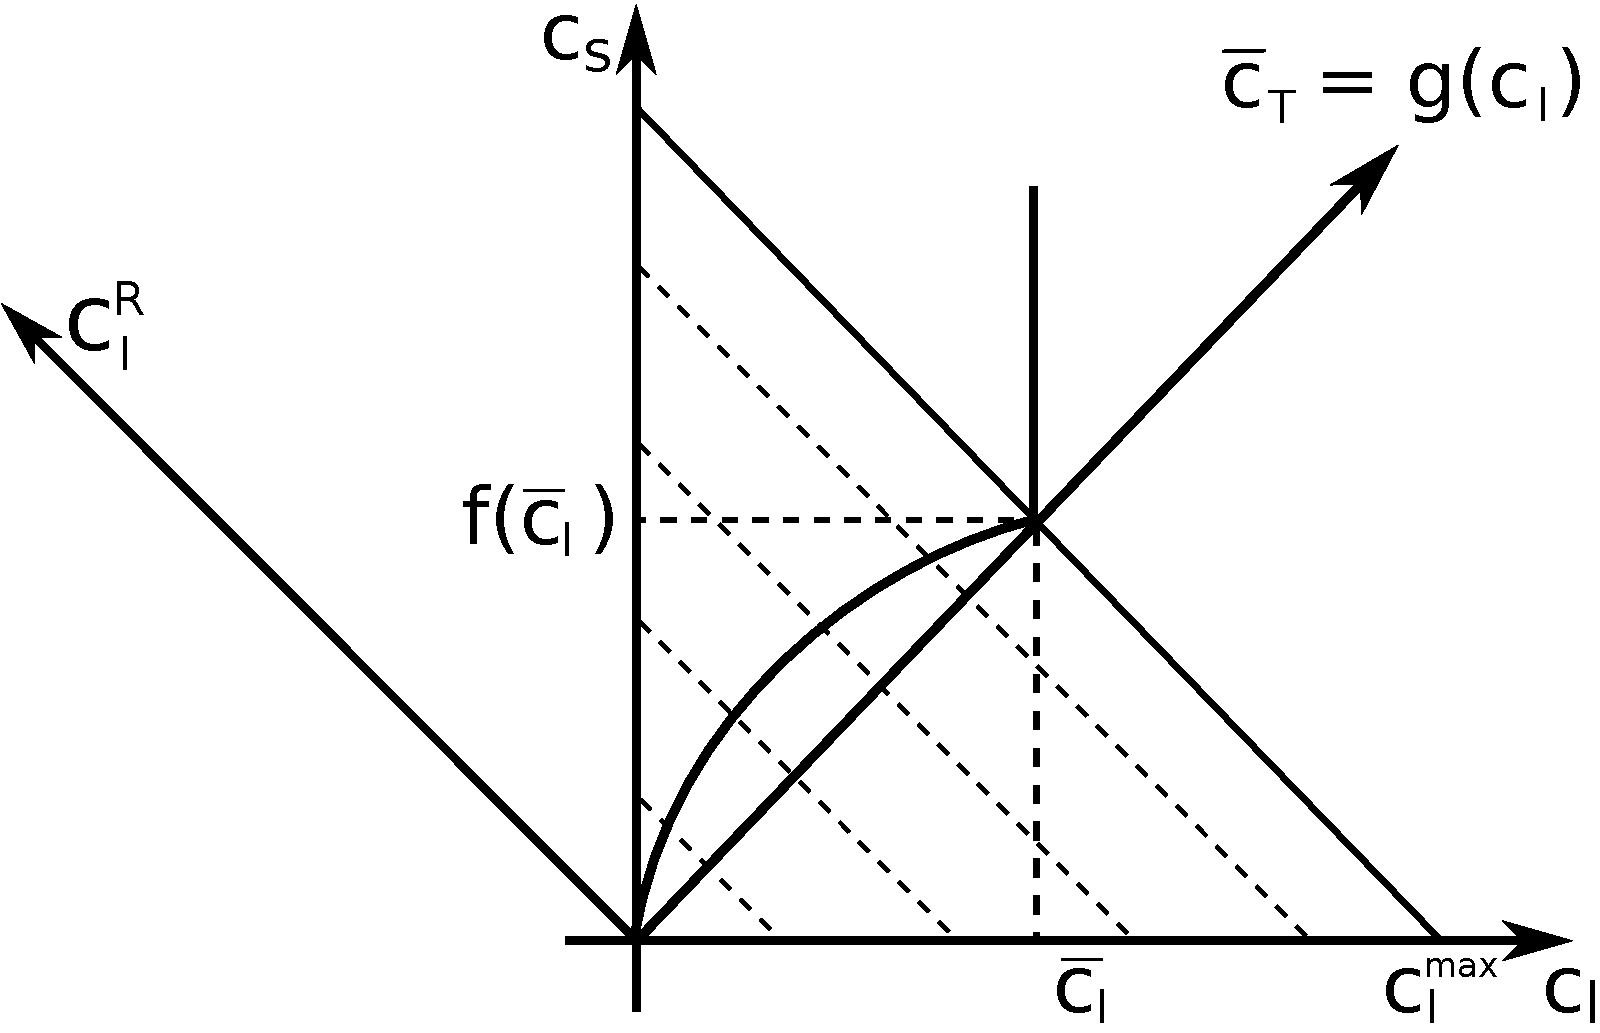
\includegraphics[width = 0.5\textwidth]{\fig/sorpce.pdf}
 \caption{Sorption in combination with limmited solubility.}
 \label{fig:sorpce}
\end{figure}


To approximate the equation \ref{eq:nonlin_sorption} using interpolation we need to prepare the set of values which represent $[c_a, f(c_a)]$, with $c_a$ equidistantly distributed in transformed (rotated and rescaled) coordination system at first. The approach for construction of interpolation table follows.
\begin{enumerate}
 \item Maximal "total mass" $konst._T^{limit} = k_a\cdot c_a^{limmit} + k_s\cdot f(c_a^{limmit})$ is computed.
 \item Total mass step is derived $mass\_step = konst._T^{limit}/n\_steps$. $n\_steps$ is equal to \hyperA{Sorptions::substeps}{$substeps$} in con-file.
 \item Appropriate $c_a^i = (mass\_step\cdot i)/k_a,~i\in \{0,\ldots, n\_steps\}$ are computed. 
 \item The equations $k_a\cdot c_a^i = k_a\cdot c_a + k_s\cdot f(c_a)~i\in \{0,\ldots, n\_steps\}$ are solved for $c_a$ as unknown. The solution is the set of ordered couples (points) $[c_a^l,f(c_a^l)],~l\in\{0,\ldots,n\_steps\}$.
\end{enumerate}
After computation of $\{[c_a^l,f(c_a^l)]\}$ we transform these coordinates to the system where total mass is independent variable. This is done by multiplication of precomputed points using transformation matrix ${\bf A}$.
\begin{equation}
 \begin{array}{l}
  \overrightarrow{c}^R = {\bf A}\cdot\overrightarrow{c}\\
  \left[\begin{array}{c} c_a^{R,l}\\ c_s^{R,l} \end{array}\right] = 
  \left[\begin{array}{cc}
    n\cdot \rho_w & M_s(1 - n)\rho_H\\
    -M_s(1 - n)\rho_H & n\cdot \rho_w
  \end{array}\right]\cdot
  \left[\begin{array}{c} c_a^l\\ c_s^l \end{array}\right]\\
  l\in\{0,\ldots,n\_steps\}
 \end{array}
 \label{eq:transf_mat}
\end{equation}

The values $c_a^{R,l}$ are equidistantly distributed and there is no reason to save them, but the values $c_s^{R,l}$ are stored in onedimensional interpolation table.

Once we have the interpolation table, we can use it for projection of ${[c_a,c_s]}$ transport results on the isotherm under concideration. The approach look as folows.
\begin{enumerate}
 \item Achieved concentrations are transformed to the coordination system through multiplication with the matrix ${\bf A}$, see \ref{eq:transf_mat}.
 \item Transrformed values are interpolated.
 \item The result of interpolation is transformed back. The backward transformation consist of multiplication with ${\bf A}^T$ which is followed by rescaling the result. Rescaling the result is neccessery because  ${\bf A}$ is not orthonormal as it is shown bellow.
 \[
 \begin{array}{l}
 {\bf A}^T\cdot{\bf A} =
  \left((n - 1)^2\cdot M_s^2\cdot \rho_h^2 + n^2\cdot \rho_w^2\right)\cdot\left[\begin{array}{cc}
    1 & 0\\
    0 & 1
  \end{array}\right]
  \end{array}
 \]
\end{enumerate}


\subsection{Limmited Solubility}\label{subsec:lim_solub}
When $k_a\cdot c_a + k_s\cdot f(c_a) > k_a\cdot c_a^{limmit} + k_s\cdot f(c_a^{limmit})$ neither iterative solver nor interpolation table is used. The aqueous concentration is set to be $c_a^{limmit}$ and sorbed concentration is computed $c_s = (k_a\cdot c_a + k_s\cdot f(c_a) - k_a\cdot c_a^{limmit})/k_s$.

\subsection{Sorption in dual porosity model} \label{subsec:sorp_dual_por}
THIS NEEDS TO BE COMPLETED AND CHECKED (TEST WITH REFERENCE DATA MUST BE CREATED)
\vspace{1cm}

There are two parameters $k_a$ and $k_s$, scale of aqueous concentration and scale of sorbed concentration, respectively.  
There is a difference in computation of these in the dual porosity model because both work on different concentrations
and different zones.

Let $c_{ma}$ and $c_{ms}$ be aqueous and sorbed concentration in mobile zone, 
$c_{ia}$ and $c_{is}$ be aqueous and sorbed concentration in immobile zone,
$\vartheta_m$ and $\vartheta_i$ be mobile and immobile porosity,
and $\varphi$ be the sorbing surface.
Further $M$ denotes molar mass, $\rho_H$ denotes rock density.

The sorbing surface in the mobile zone is given by
\begin{equation}
  \varphi = \frac{\vartheta_m}{\vartheta_m + \vartheta_i}, 
\end{equation}

while in the immobile zone it becames
\[ 1 - \varphi = 1-\frac{\vartheta_m}{\vartheta_m + \vartheta_i} = \frac{\vartheta_i}{\vartheta_m + \vartheta_i}. \]

Remind the mass balance equation (\ref{eq:mass_balance_base2}), divided by $\rho_w$ in the actual implemenation
\begin{eqnarray}
 \begin{array}{l}
  const._T = k_a\cdot c_a + k_s\cdot c_s,\\
  k_a = \vartheta, \\
  k_s = M_s \cdot\rho_H\cdot(1-\vartheta),
 \end{array}
 \label{eq:scale_params}
\end{eqnarray}
where $\vartheta = \vartheta_m + \vartheta_i$ is the porosity.
The scaling parameters are changed in the dual porosity model such that in the mobile zone
\begin{eqnarray}
 \begin{array}{l}
  const._T = k_a\cdot c_{ma} + k_s\cdot c_{ms},\\
  k_a = \vartheta_m, \\
  k_s = M_s \cdot\rho_H\cdot(1-\vartheta_m - \vartheta_i)\varphi,
 \end{array}
 \label{eq:scale_params_m}
\end{eqnarray}
and in the immobile zone
\begin{eqnarray}
 \begin{array}{l}
  const._T = k_a\cdot c_{ia} + k_s\cdot c_{is},\\
  k_a = \vartheta_i, \\
  k_s = M_s \cdot\rho_H\cdot(1-\vartheta_m - \vartheta_i)(1 - \varphi).
 \end{array}
 \label{eq:scale_params_i}
\end{eqnarray}
